\chapter{Resource Access Protocols}
\section{Introduction}
A \side{resource} is any software structure that can be used by a process to advance its executino. Tipically,  a resource can be a data structure, a set of variables, a main mamory area, a file, or a set of registers of a peripheral device. A resource dedicated to a particular process is said to be \textit{private}, whereas a resource that can be used by more tasks is called a \textit{shared resource}. A shared resource protexted against concurrent accesses is called an \textit{exclusive resource}.

To ensure consistency of the data structures in exclusive resources, any concurrent operating system should use appropriate resource access protocols to guarantee a mutual exclusion among competing tasks. A piece of code executed under mutual exclusion contraints is called a \side{critical section}.

Any task that needs to enter a critical section must wait until no other task is holding the resource. A task waiting for exclusive resource is said to be \textit{blocked} on that resource, othertwise it proceeds by entering the critical section and holds the resource. When a task leaves a critical section, the resource associated with the critical section becomes \textit{free}, and it can be allocated to another waiting task, if any.

In this chapter, we describe the main problems that may arise in a uniprocessor system when concurrent tasks use shared resources in exclusive mode, and we present some resource access protocols designed to avoid such problems and bound the maximum blocking time of each task. We then show how such blocking times can be used in the schedulability analysis to extend the guaranteee tests derived for periodic task sets.

\subsection{Atomicity}
So far we have assumed that all tasks that run and compete for a processor are independent, which means that they do not interact with one another. But there are several occasions in which this assumption cannot be made (e.g. when two tasks need to share information, exchange variables,\dots).
The other is when you have to compete for shared resources.

In this section we will introduce this problem and in particular we will introduce the notion of atomicity.
\definition{Atomic Instruction}{An atomic instruction is an instruction whose execution cannot be interleaved with the execution of other instructions}
In this sense atomic operations are always sequentialized since they cannot be interrupted. Under these conditions they are safe operations.\\
On the other hand, non atomic operations can be interrupted, and as such they are not \textit{safe} operations.

Usually, it is preferrable to have, whenever possible, non atomic operations, because they allow you to exploit in full the possibility of scheduling the processor to activities having higher priority via preemption.

\example{Non atomic operations}{
    Conside a simple operation like 
    \[x = x+1\]
    The variable is stored in a memory address that we call $x$. Hence, whenever the variable is incremented using this operation, we would have to:
    \begin{itemize}
        \item load the variable $x$ into a register $R0$
        \begin{center}
        \texttt{LD  R0, x}
        \end{center}
        \item increment the register
        \begin{center}
            \texttt{INC  R0}
        \end{center}
        \item store back the value contained in the register into $x$
        \begin{center}
        \texttt{ST  x, R0}
        \end{center}
    \end{itemize}
}
If the same operation is executed inside an interrupt handler an inconsistency may arise.

\example{Interrupt on non-atomic operations}{
Let us consider that the increment operation is both applied in the normal code and in an interrupt handler code (routine executed in response to an interrupt).\\
In both cases, the operation is translated into the assembly language using three instructions (load, increment and store).

The program starts executing as follows:
\begin{enumerate}
    \item The normal code starts executing: the value of $x$ is loaded from memory to the register
    \item At some point during this operation something triggers the execution of the interrupt
    \item The interrupt handler creates a copy of all the registers
    \item The interrupt handler load (once again) $x$ from memory, increments the register and stores the result in memory (the value of $x$ in memory has changed to $x+1$)
    \item Upon the interrupt handler has completed, the saved registers are restored. Hence, the old value of the register (i.e. $x$) is loaded back, its value is incremented to $x+1$ and stored into memory at the address of $x$ 
\end{enumerate}
The problem is that even though the code should have performed two increments (i.e. the final value should have been $x+2$), it yields the incorrect result (i.e. $x+1$).

From a logical point of view two increment operations should have taken place, but in effect one of them not successfully completed because while i was incrementing the variable, I was allowed to be interrupted and I was left with a state that was not up to date.
}

The nasty problem about this phenomenon is that it does not always happen in this way, because sometimes the function successfully completes before the interrupt is fired.\\
The example provided is the description of a condition called \side{critical race}, because you can have multiple execution of your code that interleave the operation in slightly different ways and you obtain different results.

This is a nasty problem in computer science because it might not materialize for years.

This is so because you cannot make assumption about the speed of the hardware and on the exact moment when certain events take place (we do not know the order of execution of the hardware instructions).

The case studies proposed are a perfect example of a not atomic operation that should be atomic.

The same behaviour occurs not only in the case of interrupts but also on interleaving tasks: so you could have two tasks running in parallel, both of which are sharing the variable $x$.

We can give a few definitions that are important for the follow up of our discussion:
\definition{Shared Object}{An object where the conflict may happen.}
\definition{Critical section}{A critical section is a sequence of operations that cannot be interleaved with other operations on the same resource}
\definition{Mutual exclusion}{Two critical sections cannot be active at the same time (they must be sequentialized). Either one or the other needs to stand by while the other executes}

There are three ways to obstain mutual exclusion:
\begin{enumerate}
    \item Implementing the critical section as an atomic operation.\\
    This that interrupt are disabled before the execution of the critical section and then are restored upon termination of the operation. The problem with this is that it is really tough because disabling the interrupts the I/O system of the machine is no longer allowed to work properly. (pressing an emergency button will have no effect and the execution of the code will continue),\\
    Moreover if the critical section is long, no interrupt can arrive during the critical section. In the case of a timer interrupt that arrives every 1ms, if a critical section lasts more than 1ms, a timer interrupt could be lost!
    \item Disabling the preemption (system-wide).\\
    This strategy will have some problems, because all the tasks will suffer from this suspention of the preemption even though they do not use shared resources.
    \item Selectively disabling the preemption (using semaphores and mutual exclusion).\\
    This strategy will disable preemption only for the task that operates on the shared resource.
\end{enumerate}
Hence, we should try to disable preemption rather than disabling interrupts.

Still the big issue with selectively disabling preemption the priority mechanism is no longer enforced: during the critical section might force the process to execute low priority tasks because preemption is disabled. This phenomenon is known as \side{Priority Inversion}.

If Priority inversion is not correctly managed it may lead to a complete violation of all timing contraints.
\subsection{Interacting Tasks}
Until now, we have considered only independent tasks, which are characterized by the fact that a job never blocks or suspends and a task only blocks on job termination.\\
In the real world, jobs might block for various reasons:
\begin{itemize}
    \item Tasks exchange data throught shared memory (mutual exclusion)
    \item A task might need to synchronize with other tasks while waiting for some data
    \item A job might need a hardware resource which is currently not available.
\end{itemize}

\example{Control Application}{
    Let us consider a control application composed by three periodic tasks:
    \begin{itemize}
        \item $\tau_1$ reads the data from the sensors and applies a filter. The results are stored in memory.
        \item $\tau_2$ reads the filtered data and computes some control law (updating the state and the outputs); both the state and the outputs are stored in memory
        \item $\tau_3$ reads the outputs and writes on an actuator
    \end{itemize}
    All of the three tasks access data in shared memory. This means that there are conflicts on accessing this data concurrently with the risk that the data structures become inconsistent.
    }

\subsection{Priority Inversion Phenomenon}

The rest of this chapter presents the following resource access protocols:
\begin{itemize}
    \item Non-Preemptive Protocol (NPP)
    \item Highest Locking Priority (HLP)
    \item Priority Inheritance Protocol (PIP)
    \item Priority Ceiling Protocol (PCP)
\end{itemize}


\section{Non Preemptive Protocol (NPP)} 
A simple solution that avoids the unbounded priority inversion problem is to disallow preemption during the execution of any critical section. This method, also referred to as \side{Non-Preemptive Protocol (NPP)}, can be implemented by raising the priority of a task to the highest priority level whenever it enters a shared resource. In particular, as soon as a task $\tau_i$ enters a resource $R_k$, its dynamic priority is raised to the level:
\[p_i(R_k) = \max_h \{p_h\}\]
The dynamic priority is then reset to the nominal value $p_i$ when the task exits the critical section.

\begin{figure}[!h]
    \centering
    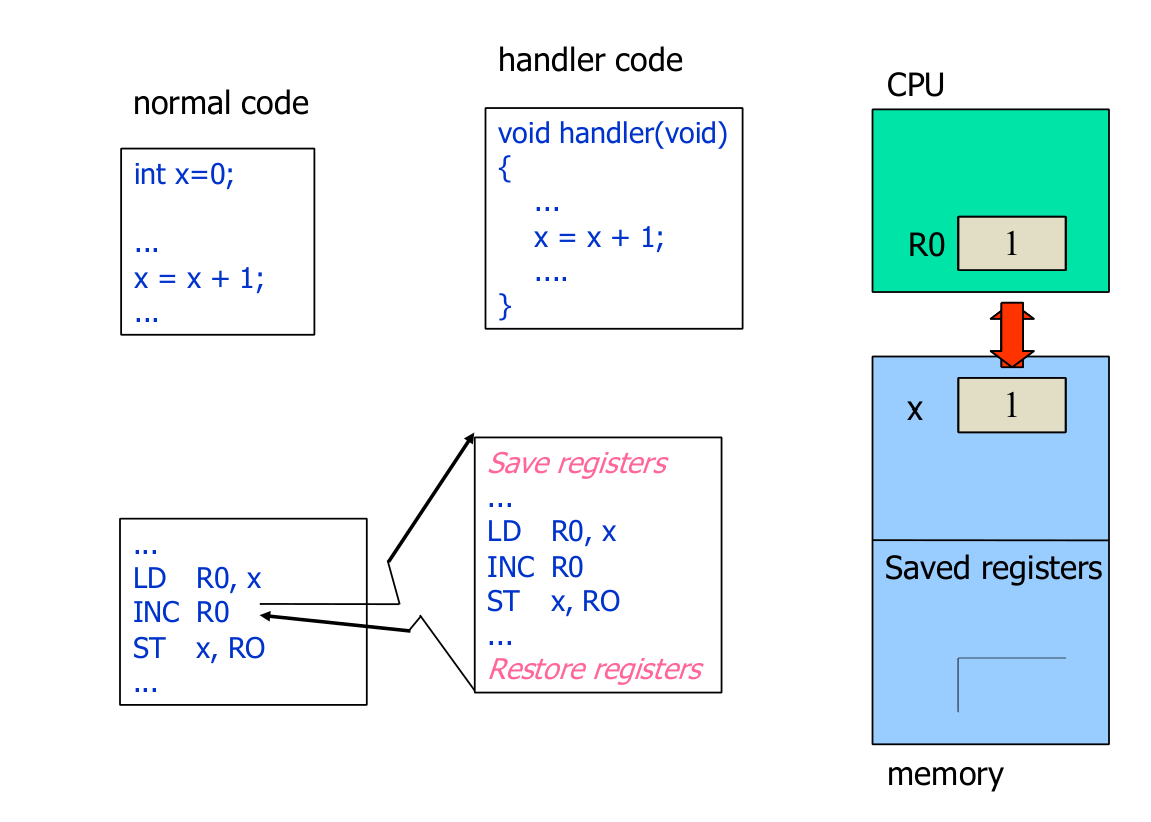
\includegraphics[width =0.75\textwidth]{images/image06.png}
\end{figure}


This method solves the priority inversion phenomenon, however, is only appriopriate when tasks use short critical sections because it creates unnecessary blocking. This actually might cause deadline misses of tasks that do not use the shared resource.

\begin{figure}[!h]
    \centering
    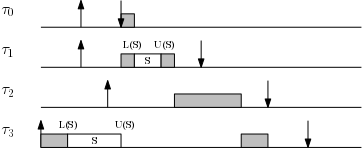
\includegraphics[width =0.75\textwidth]{images/image07.png}
\end{figure}
In the example, $\tau_0$ misses its deadline (suffers a blocking time equal to 3) even though it does not use any resource!!\\
The solution is to raise $\tau_3$ priority to the maximum between tasks accessing the shared resource (i.e. $\tau_1$) priority.

\subsection{Blocking Time and Response Time}
NPP introduces a blocking time on all tasks bounded by the maximum length of a critical section used by lower priority tasks.
Such blocking time affect the response times of the task as follows:
\[R_i = C_i + B_i + \sum_{j=1}^{i-1} \ceil{\cfrac{R_i}{T_j}}C_j\]
where:
\begin{itemize}
    \item $B_i$ is the blocking time from lower priority tasks
    \item $\sum_{h=1}^{i-1} \ceil{\cfrac{R_i}{T_h}}C_h$ is the interference from higher priority tasks
\end{itemize}
\example{Response time computation}{
Consider the following task set:
\begin{itemize}
    \item $\tau_1 = (20, 30, 70)$ accessing resource for $\xi_{1,1} = 0$ units of time
    \item $\tau_2 = (20, 45, 80)$ accessing resource for $\xi_{2,1} = 1$ units of time
    \item $\tau_3 = (20, 130, 200)$ accessing resource for $\xi_{3,1} = 2$ units of time
\end{itemize}

It follows that the blocking times associated with each task is the maximum length of a critical section used by lower priority tasks:
\begin{itemize}
    \item $B_1 = 2$ since $\tau_3$ might block the task for 2 units of time when accessing its resource
    \item $B_2 = 2$ since $\tau_3$ might block the task for 2 units of time when accessing its resource
    \item $B_3 = 0$ since there are no lower priority tasks that can block it
\end{itemize}
Thus, the response time of each task takes the form 
\[R_i = C_i + B_i + \sum_{j=1}^{i-1} \ceil{\cfrac{R_i}{T_j}}C_j\]
\begin{itemize}
    \item For $\tau_1$
    \begin{align*}
        R_1^{(0)} &= 20 + 2 = 22
    \end{align*}
    \item For $\tau_2$
    \begin{align*}
        R_2^{(0)} &= 20 + 2 = 22\\
        R_2^{(1)} &= 20 + 2 + \ceil{\cfrac{22}{70}}20 = 42\\
        R_2^{(2)} &= 20 + 2 + \ceil{\cfrac{42}{70}}20 = 42
    \end{align*}
    \item For $\tau_2$
    \begin{align*}
        R_3^{(0)} &= 35 + 0 = 35\\
        R_3^{(1)} &= 35 + 0 + \ceil{\cfrac{35}{70}}20 + \ceil{\cfrac{35}{80}}20 = 75\\
        R_3^{(1)} &= 35 + 0 + \ceil{\cfrac{75}{70}}20 + \ceil{\cfrac{75}{80}}20 = 95\\
        R_3^{(1)} &= 35 + 0 + \ceil{\cfrac{95}{70}}20 + \ceil{\cfrac{95}{80}}20 = 115\\
        R_3^{(1)} &= 35 + 0 + \ceil{\cfrac{115}{70}}20 + \ceil{\cfrac{115}{80}}20 = 115
    \end{align*}
\end{itemize}

}

\section{Highest Locking Priority (HLP)}
The \side{Highest Locking Priority (HLP)} protocol improves NPP by raising the priority of a task that enters a resource $R_k$ to the highest priority among the tasks sharing that resource. In particular as soon as a task $\tau_i$ enters a resource $R_k$, its dynamic priority is raised to the level
\begin{equation}
\label{eq:equation2}
p_i(R_k) = \max_h\{p_i | \tau_h \text{ uses } R_k\}
\end{equation}

The dynamic priority is then reset to the nominal value $p_i$ when the task exits the critical section. The online computation of the priority level in equation \ref{eq:equation2} can be simplified by assigning each resource $R_k$ a \side{priority ceiling} $C(R_k)$ (computed offline) equal to the maximum priority of the tasks sharing $R_k$; that is:
\[C(R_k) = \max_h\{p_i | \tau_h \text{ uses } R_k\}\]
Then, as soon as a task $\tau_i$ enters a resource $R_k$, its dynamic priority is raised to the ceiling of the resource. For this reason, this protocol is also referred to as \side{Immediate Priority Ceiling}.

\begin{figure}[!h]
    \centering
    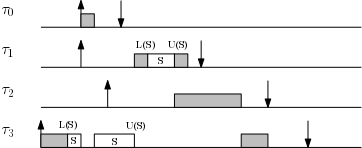
\includegraphics[width =0.75\textwidth]{images/image08.png}
\end{figure}
The main problem with HLP is that we must know in advance which task will access the resource: hence you need to have a complete control over the application, and how the application is written. Because knowing the code is the only way to know which resources is going to use. So this mechanism works very well if you have full control of what is running in your PC or embedded system.

\section{Priority Inheritance Protocol (PIP)}
The \side{Priority Inheritance Protocol (PIP)} proposed by Sha, Rajkumar and Lehoczky, avoids unbounded priority inversion by modifying the priority of those tasks that cause blocking. In particular, when a task $\tau_i$ blocks one or more higher-priority tasks, it temporarily assumes (\textit{inherits}) the highest priority of the blocked tasks. This prevents medium-priority tasks from preempting $\tau_i$ and prolonging the blocking duration experienced by the higher-priority tasks.

The Priority Inheritance Protocol can be defined as follow:
\begin{itemize}
    \item Tasks are scheduled based on their active priorities. Tasks with the same priority are executed in a First Come First Served discipline.
    \item When task $\tau_i$ tries to enter a critical section and resource $R_k$ is already held by a lower-priority task $\tau_j$, then $\tau_i$ is blocked. $\tau_i$ is said to be blocked by the task $\tau_j$ that holds the resource. Otherwise, $\tau_i$ enters the critical section.
    \item When a task $\tau_i$ is blocked, it transmits its active priority to the task $\tau_j$ that holds the semaphore/mutex. Hence, $\tau_j$ resumes adn executes the rest of its critical section with a priority $p_j = p_i$. Task $\tau_j$ is said to inherit the priority of $\tau_i$. In general, a task inherits the highest priority of the tasks it blocks. That is, at every instant,
    \begin{equation}
        \label{eq:equation3}
        p_j(R_k) = \max \{P_j, \max_h \{P_h | \tau_h \text{ is blocked on }R_k\}\}
    \end{equation}
    \item When $\tau_j$ exits a critical section, it unlocks the mutex/semaphore, and the highest-priority task blocked, if any, is awakened. Moreover, the avtive priority of $\tau_j$ is updated as follows: if no other tasks are blocked by $\tau_j$, $p_j$ is set to its nominal priority $P_j$; otherise it is set to the highest priority of the tasks blocked by $\tau_j$, according to equation \ref{eq:equation3}.
    \item Priority inheritance is transitive; that is, if a task $\tau_3$ blocks a task $\tau_2$, and $\tau_2$ blocks a task $\tau_1$, then $\tau_3$ inherits the priority of $\tau_1$ via $\tau_2$
\end{itemize}

A high priority task can experience two kinds of blocking: \side{Direct blocking} and \side{Push-through blocking}.


\definition{Direct blocking}{It occurs when a higher-priority task tries to acquire a resource already held by a lower-priority task. Direct blocking is necessary to ensure the consistency of the shared resources}
\definition{Push-through blocking}{It occurs when a medium-priority task is blocked by a low-priority task that has inherited a higher priority from a task it directly blocks. Push-through blocking is necessary to avoid unbounder priority inversion}

\begin{figure}[!h]
    \centering
    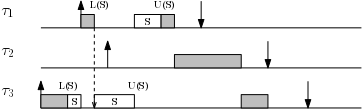
\includegraphics[width =0.75\textwidth]{images/image09.png}
\end{figure}

Although the Priority Inheritance Protocol bounds the priority inversion phenomenon, the blocking duration for a task can still be substantial because a chain of blocking can be formed. Another problem is that protocol does not prevent deadlocks (however, the latter problem can be solved by imposing a total ordering on the mutex accesses).

\subsection{Blocking time and computation time}
For the Priority inheritance protocol we only consider non nested critical sections. In fact, in presence of multiple inheritance, the computatino of the blocking time becomes very complex, whereas in non nested critical sections, multiple inheritance cannot happend and the computation of the blocking time becomes simpler.

The maximum blocking time can be computed based on two important properties which provide an upper bound on the number of times a task can block.
\theorem{}{If PI is used, a task block only once on each different critical section}
\theorem{}{If PI is used, a task can be blocked by another lower priority task for at most the duration of one critical section}
These two properties imply that a task can be blocker more than once, but only once per each resource and once by each task.

The Blocking time computation makes use of a \side{resource usage table}:
\begin{itemize}
    \item A task per row, in decrasing order of priority
    \item A resource per column
    \item Cell $(i,j)$ contains $\xi_{i,j}$, i.e. the lenght of the longest critical section of task $\tau_i$ on resource $S_j$, or 0 if the task does not use the resource.
\end{itemize}

The computation of the blocking time makes use of the resource usage table and follows the following procedure (taking into considerations the two PI properties):
\begin{itemize}
    \item A task can be blocked only by lower priority tasks: then, for each task (row), we must consider only the rows below (tasks with lower priority)
    \item A task block only on resources directly used, or used by higher priority tasks (\side{indirect blocking}): for each task, only consider columns on which it can be blocked (used by itself or by higher priority tasks)
\end{itemize}

Let us consider the following resource usage table:
\begin{table}[!h]
    \centering 
    \begin{NiceTabular}[hvlines]{cccc}
        & $S_1$& $S_2$& $S_3$\\
        $\tau_1$&2&0&0\\
        $\tau_2$&0&1&0\\
        $\tau_3$&0&0&2\\
        $\tau_4$&3&3&1\\
        $\tau_5$&1&2&1
    \end{NiceTabular}
\end{table}

\example{}{
    \begin{itemize}
        \item $B_1$\\
        $\tau_1$ can be blocked only on $S_1$. Therefore, we must consider only the first column, and take the maximu, which is 3.\\
        Therefore $B_1 = 3$.
        \item $B_2$\\
        $\tau_2$ can be blocked on $S_1$ (indirect blocking) by lower priority tasks inheriting a higher priority and on $S_2$ by lower priority tasks.\\
        Consider all cases where two distinct lower priority tasks in $\{\tau_3, \tau_4,\tau_5\}$ access $S_1$ and $S_2$, sum the two contributions, and take the maximum:
        \begin{itemize}
            \item $\tau_4$ on $S_1$ and $\tau_5$ on $S_2$: blocking time of 5
            \item $\tau_4$ on $S_2$ and $\tau_5$ on $S_1$: blocking time of 4
        \end{itemize}
        Hence, $B_2 = 5$
        \item $B_3$\\
        $\tau_3$ can be blocked on all 3 resources
        \begin{itemize}
            \item $\tau_4$ on $S_1$ and $\tau_5$ on $S_2$: blocking time of 5
            \item $\tau_4$ on $S_1$ and $\tau_5$ on $S_3$: blocking time of 4
            \item $\tau_4$ on $S_2$ and $\tau_5$ on $S_1$ or $S_3$: blocking time of 4
            \item $\tau_4$ on $S_3$ and $\tau_5$ on $S_2$: blocking time of 3
            \item $\tau_4$ on $S_3$ and $\tau_5$ on $S_1$: blocking time of 2
        \end{itemize}
        Hence, $B_3 = 5$
        \item $B_4$\\
        $\tau_4$ can be blocked on all 3 resources, since it can be blocked only by $\tau_5$
        \begin{itemize}
            \item $\tau_5$ on $S_2$: blocking time of 2
            \item $\tau_5$ on $S_1$ or $S_3$: blocking time of 1
        \end{itemize}
        Hence, $B_4 = 2$
        \item $\tau_5$ cannot be blocked by any other task (because it is the lower priority task).\\
        Hence, $B_5 = 0$
    \end{itemize}
}

As usual the schedulability tests with a blocking time can be carried on using the three tests that we have seen:
\begin{itemize}
    \item Processor utilization factor test.\\
    The system is schedulable if
    \[\forall i \in [1,n]\qquad \sum_{k=1}^{i-1}\cfrac{C_k}{T_k} + \cfrac{C_i + B_i}{T_i} \le i(2^{\sfrac{1}{i}} - 1)\]
    \item Response time analysis
    \[R_i = C_i + B_i + \sum_{h=1}^{i-1}\ceil{\cfrac{R_i}{T_h}}C_h\]
    \item Processor demand analysis.\\
    In a task set $\mathcal{T}$ composed of independent and periodic tasks, $\tau_i$ is schedulable (for all possible phasing) if and only if
    \[\exists t\in [0,D_i]\qquad W_i(0,t) = C_i + \sum_{h=1}^{i-1} \ceil{\cfrac{t}{T_h}}C_h \le t-B_i\]
    As usual we can define
    \[W_i(t) =C_i + \sum_{h=1}^{i-1} \ceil{\cfrac{t}{T_h}}C_h\]
    \[L_i(t) = \cfrac{W_i(t)}{t}\]
    \[L_i = \min_{t\in [0,D_i]}L_i(t) + \cfrac{B_i}{t}\]
    The task set is schedulable if $\forall i$, $L_i\le 1$.\\
    Again, we can compute $L_i$ by only considering the scheduling points.
\end{itemize}

\section{Priority Ceiling Protocol (PCP)} % follow lecture
The \side{Priority Ceiling Protocol (PCP)} was introduced by Sha, Rajkumar, and Lehoczky to bound the priority inversion phenomenon and prevent the formation of deadlocks and chained blocking.

The basic idea of this method is to extend the Priority Inheritance Protocol with a rule granting a lock request on a free mutex. To avoid multiple blocking, this rule does not allow a task to enter a critical seciton if there are locked mutexes that could block it. This means that once a task enters its first critical section, it can never be blocked by lower-priority tasks until its completion.

In order to realize this idea, each mutex is assigned a priority ceiling equal to the highest priority of the tasks that can lock it. Then, a task $\tau_i$ is allowed to enter a critical section only if its priority is higher than all priority ceiling of the mutexes currently locked by tasks other than $\tau_i$.

The problem with Priority Inheritance Protocol resides in the case where there are multiple blockings. 

\begin{figure}[!h]
    \centering
    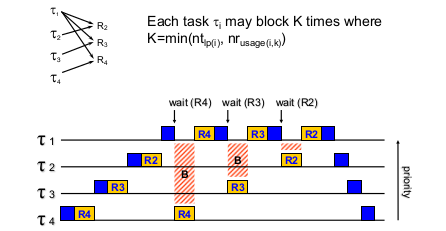
\includegraphics[width=.75\textwidth]{images/image11.png}
\end{figure}

\example{Multiple Blocking}{Consider a task set of four tasks ($\tau_1, \tau_2, \tau_3, \tau_4$) sharing three resources $R_2, R_3, R_4$ in the following manner:
\begin{itemize}
    \item $\tau_1$ uses $R_2, R_3, R_4$
    \item $\tau_2$ uses $R_2$
    \item $\tau_3$ uses $R_3$
    \item $\tau_4$ uses $R_4$
\end{itemize}
Now consider the following case:
\begin{enumerate}
    \item The schedule starts executing $\tau_4$
    \item The task enters the critical section and locks resource $R_4$.
    \item $\tau_4$ is preempted, and $\tau_3$ starts executing (higher priority task)
    \item $\tau_3$ enters a critical section and locks resource $R_3$.
    \item $\tau_3$ is preempted, and $\tau_2$ starts executing (higher priority task)
    \item $\tau_2$ enters a critical section and locks resource $R_2$.
    \item $\tau_2$ is preempted, and $\tau_1$ starts executing (higher priority task)\\
At this point all three resources are locked by the three lower priority tasks
    \item whenever $\tau_1$ tries to access any of the three resources it is blocked and have to give back the execution to the task holding the resource. 
\end{enumerate}
In the case described above, the protocol perform three context switches between an high priority task and a lower priority task holding the resource introducing unnecessary blocking time to task $\tau_1$ and performing too many context switches (which are expensive from a real-time perspective, to be precise 2 context switches for each blocking time).\\
In addition, the lower priority tasks preempted are active all the time, and therefore they allocate on the stack their local variable. Within the stack we would have all the cumulative use of memory of each task at the same time.
}

Hence we can notice that Priority Inheritance Protocol brings several drawbacks:
\begin{itemize}
    \item Tasks may block multiple times
    \item Worst case behaviour even worse that non-preemptable critical section
    \item Costly implementation except for very simple cases
    \item Does not even prevent deadlocks.
\end{itemize}

For all these reasons, priority ceiling was proposed.
\definition{Priority ceiling of a resource $S$}{Maximum priority among all tasks that can psssibly access $S$}
The mechanism behind the Priority Ceiling Protocol is that a process can only lock a resource if its dynamic priority is higher than the ceiling of any currently locked resource (excluding any that it has already locked itself).
Thus if task $\tau$ blocks, the task holding the lock on the blocking resource inherits its priority.

There are two forms of Priority Ceiling Protocol:
\begin{itemize}
    \item Original Priority Ceiling Protocol (OPCP)
    \item Immediate Priority Ceiling Protocol (IPCP)
\end{itemize}

The nice priorities of both these protocols are:
\begin{itemize}
    \item A high priority process can be blocked at most once during its execution by lower priority processes
    \item Deadlocks are prevented
    \item Transitive blocking is prevented, hence multiple inheritance cannot happen
\end{itemize}


\subsection{Original Priority Ceiling Protocol (OPCP)}

\begin{figure}[!h]
    \centering
    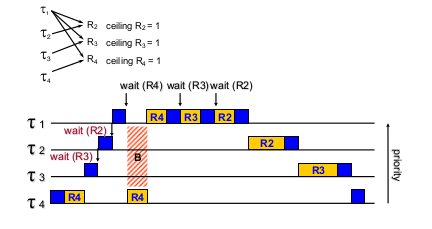
\includegraphics[width=.75\textwidth]{images/image12.png}
\end{figure}

\example{Original Priority Ceiling Protocol}{
    Consider a task set of four tasks ($\tau_1, \tau_2, \tau_3, \tau_4$) sharing three resources $R_2, R_3, R_4$ in the following manner:
\begin{itemize}
    \item $\tau_1$ uses $R_2, R_3, R_4$
    \item $\tau_2$ uses $R_2$
    \item $\tau_3$ uses $R_3$
    \item $\tau_4$ uses $R_4$    
\end{itemize}
Given this resource utilization graph we can notice that all three resources have a priority ceiling of 1 since all three resources are used by task $\tau_1$ with the highest priority among all the tasks.

Now consider the following case:
\begin{enumerate}
    \item The schedule starts executing $\tau_4$
    \item The task enters the critical section and locks resource $R_4$.
    \item $\tau_4$ is preempted, and $\tau_3$ starts executing (higher priority task)
    \item $\tau_3$ executes and tries to lock resource $R_3$, but the protocol prevents it from locking the resource. This is because their priority of $\tau_3$ is lower than the Priority ceiling of resource $R_4$
    \item $\tau_2$ executes and tries to lock resource $R_2$, but the protocol prevents it from locking the resource. This is because their priority of $\tau_2$ is lower than the Priority ceiling of resource $R_4$
    \item $\tau_1$ executes and tries to lock resource $R_4$, but the protocol prevents it from locking the resource. It then transmits its priority to $\tau_4$
    \item $\tau_4$ resumes its utilization of $R_4$ and unlocks the resource
    \item At this point $\tau_1$ is the highest priority and can lock resource $R_4$, as well as the other resources.
\end{enumerate}
We can see that the priority ceiling on resource $R_4$ prevented task $\tau_2$ and $\tau_3$ from locking resources $R_2$ and $R_3$. 
}
This process allows to lock only once on one resource. Hence there are no excessive context switches and blocking time but still the stack occupation of the active tasks is the same.

\subsection{Immediate Priority Ceiling Protocol (IPCP)}

The Immediate priority ceiling considers the case where high and low priority tasks share a critical seciton. Still the ceiling is the highest priority among all tasks that can use the resource but this time not only a task is not allowed to occupy a resource if the priority is lower than the ceiling of any locked resource, but the task is not even allowed to start.

\begin{figure}[!h]
    \centering
    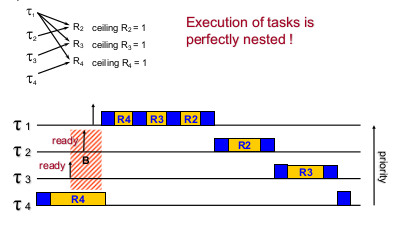
\includegraphics[width=.75\textwidth]{images/image13.png}
\end{figure}

\example{Immediate Priority Ceiling Protocol}{
    In the example proposed before:
    \begin{enumerate}
        \item The schedule starts executing $\tau_4$
        \item The task enters the critical section and locks resource $R_4$.
        \item Task $\tau_3$ (and $\tau_2$, $\tau_1$) tries to execute, but the protocol prevents it from doing so because its priority is lower than the priority ceiling of the locked resource
        \item Hence $\tau_4$ continues to utilize resource $R_4$ and upon releasing it, task $\tau_1$ has the highest priority among all tasks and can utilize all three resources without context switches.
    \end{enumerate}
}
The immediate priority ceiling protocol prevents deadlocks, excessive context switches and blocking time and considerably lowers the stack occupation of the active tasks since they are reduced (they are not even allowed to execute)

\subsection{OPCP vs IPCP}
The comparison between the two protocols is as follows:
\begin{itemize}
    \item The worst case behaviour is identical from a scheduling point of view
    \item IPCP is easier to implement than the original OPCP as blocking relationships need not to be monitored
    \item IPCP leads to less context switches as blocking is prior to first execution
    \item IPCP requires more priority movements as this happens with all resource usages; OPCP only changes priority if an actual block has occurred
    \item IPCP allows substantial savings of stack occupation
\end{itemize}

\subsection{Blocking time computation}
Contrary to priority inheritance protocol, where the blocking time is the higher combination of resource utilization between the lower rows of the resource utilization table.\\
Whereas the Priority Ceiling Protocol only considers the maximum value of the submatrix of the lower rows of the resource utilization table.

